\section{Zimny start}\label{chapter:results_cold_start}

\begin{figure}[h]
    \centering
    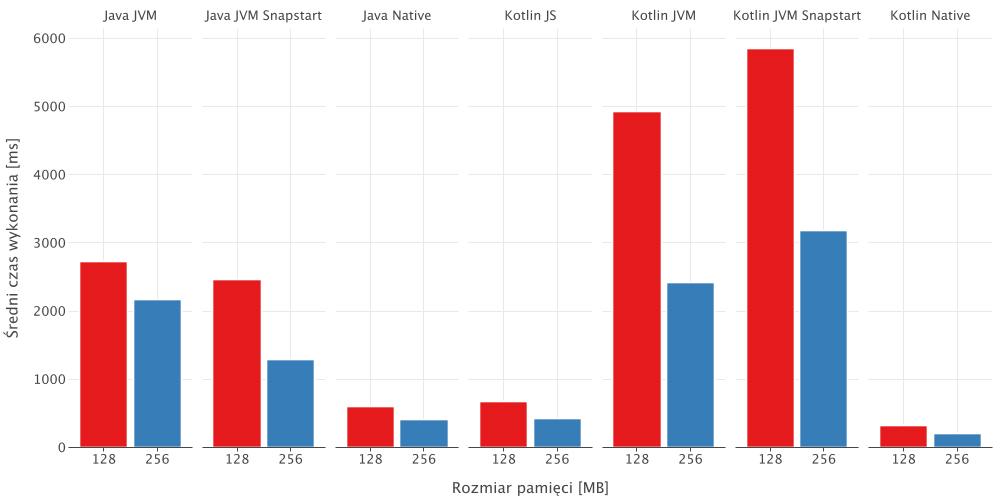
\includegraphics[width=0.95\textwidth]{charts/results/avg-cold-start-128-256.png}
    \caption{Średni czas wykonywania funkcji (zimny start) dla rozmiarów pamięci: 128 MB, 256 MB  [źródło: opracowanie własne]}
    \label{fig:avg_cold_start_128_256}
\end{figure}

\begin{figure}[h]
    \centering
    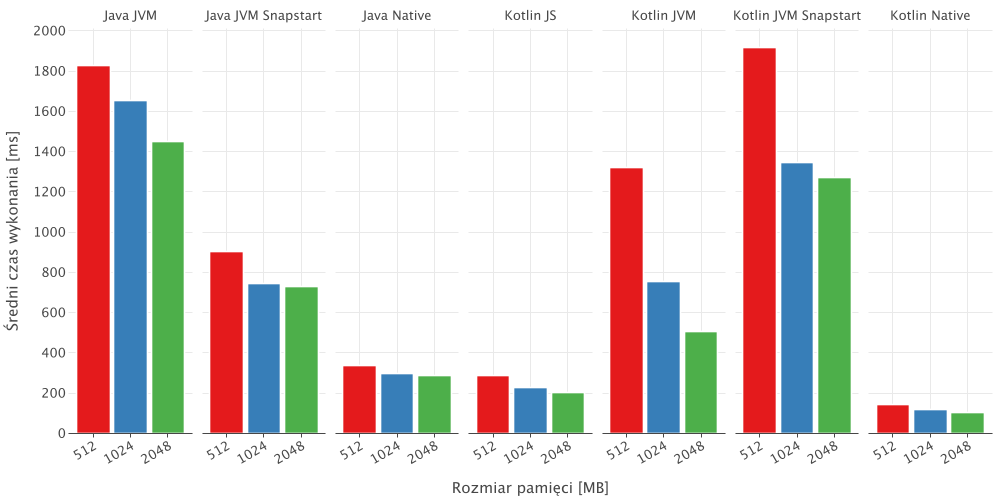
\includegraphics[width=0.95\textwidth]{charts/results/avg-cold-start-512-2048.png}
    \caption{Średni czas wykonywania funkcji (zimny start) dla rozmiarów pamięci: 512 MB, 1024 MB, 2048 MB  [źródło: opracowanie własne]}
    \label{fig:avg_cold_start_512_2045}
\end{figure}

% --- Row 1: 256 MB and 1024 MB charts ---
\begin{figure}[htbp]
    \centering % Center the minipages on the line
    \begin{minipage}[t]{0.48\textwidth} % [t] for top alignment
        \centering % Center content within this minipage
        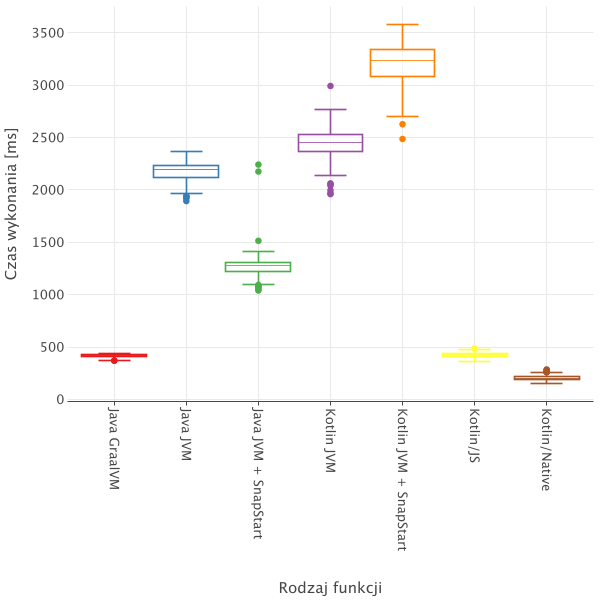
\includegraphics[width=\linewidth]{charts/results/cold-start-boxplot-256.png}
        \captionof{figure}{Czas wykonania funkcji (zimny start, 256 MB) [źródło: opracowanie własne]}
        \label{fig:cold_start_128} % Unique label for this figure
    \end{minipage}% <--- % is important
    \hfill % Space between minipages
    \begin{minipage}[t]{0.48\textwidth}
        \centering
        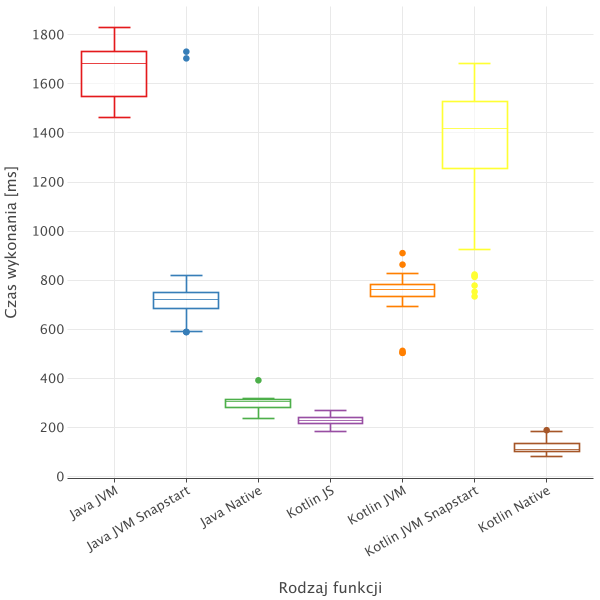
\includegraphics[width=\linewidth]{charts/results/cold-start-boxplot-1024.png}
        \captionof{figure}{Czas wykonania funkcji (zimny start, 1024 MB) [źródło: opracowanie własne]}
        \label{fig:cold_start_256} % Unique label
    \end{minipage}
    % No overall \caption for this outer figure environment, as it's just for layout.
\end{figure}
